\documentclass[../Main.tex]{subfiles}


\begin{document}
%En esta sección abordaremos los resultados de la generación de números pseudoaleatorios a través de tres metodologías distintas: la regla 30, el mapeo tienda y el mapeo logístico. En cada una de las implementaciones veremos las características, tanto gráficas teóricas como de los datos obtenidos, usando sus histogramas, momentos, función generadora y función característica. Los programas están disponibles para su inspección en el repositorio público: \cite{Lince2024}
\chapteropening{E}{n} esta sección abordaremos los resultados de la generación de números pseudoaleatorios a través de tres metodologías: la regla 30, el mapeo tienda y el mapeo logístico. En cada caso examinaremos tanto las representaciones teóricas como los resultados numéricos obtenidos mediante histogramas, momentos, función generadora y función característica. Asimismo, estudiaremos numéricamente las propiedades de convergencia de los mapeos discretos: en el mapeo tienda veremos que la distribución uniforme es atractora en $[0,1]$, mientras que en el mapeo logístico observaremos que la distribución $Beta(\tfrac{1}{2},\tfrac{1}{2})$ se comporta como atractora. Los programas están disponibles para su inspección en el repositorio público: \cite{Lince2024}.
\section{Regla 30}
Implementando la regla 30 con parámetros del sistema dinámico $n=m=1000$ 
% con cada bloque correspondiente a una variable aleatoria Bernoulli con prametro $p = \frac{1}{2}$
obtenemos resultados como la Figura \ref{fig:R30} donde podemos apreciar gráficamente la ``aleatoriedad'' (espacios en negros se distribuyen uniforme) en ambas direcciones, tanto en columnas como en renglones.
% regla 30 1000 x 1000 
\begin{figure}[h!]
    \centering
    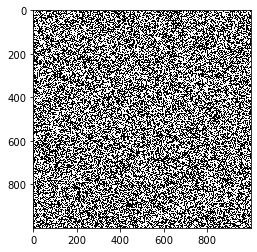
\includegraphics[width=8cm]{Tesis UNAM/graficas/R30/regla 30.png}
    \caption{Mapeo de la regla 30 de tamaño 1000(condición inical) por 1000(iteraciones).}
    \label{fig:R30}
\end{figure} 
\subsection{Uniformidad}
\subsubsection{Histogramas}
Codificando los renglones y columnas a los respectivos números en el intervalo $[0,1]$ obtenemos histogramas como los de la Figura \ref{fig:hist_R30} pudiendo apreciar a primera vista que las columnas tienen un mejor desempeño. 

% histogramas
\begin{figure}[h!]
\hfill
\subfigure[Columnas]{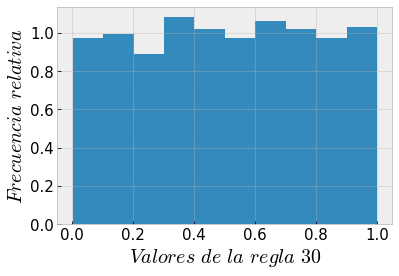
\includegraphics[width=0.49\textwidth]{Tesis UNAM/graficas/R30/Uniformidad/muestra_col.png}}
\hfill
\subfigure[Filas]{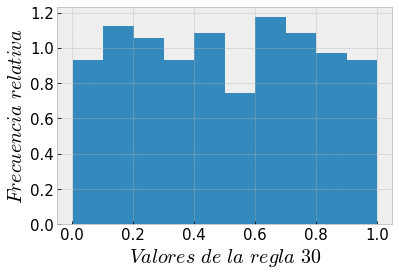
\includegraphics[width=0.49\textwidth]{Tesis UNAM/graficas/R30/Uniformidad/muestra_fila.png}}
\hfill
\caption{Histogramas de los datos generados.}
\label{fig:hist_R30}
\end{figure}
\subsubsection{Momentos}
La evaluación de un método para generar números aleatorios puede recurrir a la comparación de los momentos como lo hace \cite{Logistic Map: A Possible Random Number
Generator}.En la Figura \ref{fig:momentos_R30} se reportan los momentos de ambos conjuntos de datos; filas y columnas, así como el momento teórico. La segunda gráfica nos permite apreciar una ligera mejora en los momentos de orden mayor en los datos correspondientes a las columnas. Observemos que la mejora es de orden $10^{-3}$.

% \duda{Es significativo cuando aumentas la dimensión del cuadrado de la regla 30?}
% Momentos
\begin{figure}[h!]
\hfill
\subfigure{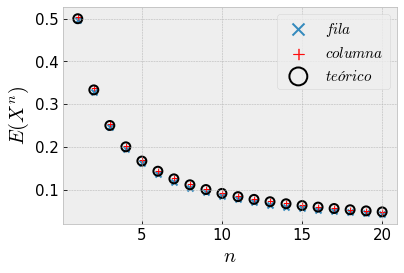
\includegraphics[width=0.49\textwidth]{Tesis UNAM/graficas/R30/Uniformidad/momentos_r30.png}}
\hfill
\subfigure{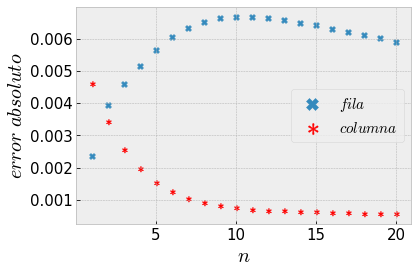
\includegraphics[width=0.49\textwidth]{Tesis UNAM/graficas/R30/Uniformidad/ErrorMomentos_r30.png}}
\hfill
\caption{Comparacion de los momentos y el error absoluto.}
\label{fig:momentos_R30}
\end{figure}

\subsubsection{Función Generadora de Momentos}
Comparando la Función Generadora de Momentos con los datos podemos obtener la Figura \ref{fig:FGM_R30} en la cual  tenemos dos escalas para analizar los datos. En el lado izquierdo de las gráficas tenemos la escala usual, mientras que en el lado derecho tenemos una escala logarítmica. Aquí, confirmamos que las columnas tienen un mejor desempeño para valores de $t$ mayores a dos.

% Funcion Generadora de Momentos
\begin{figure}[h!]
\hfill
\subfigure
{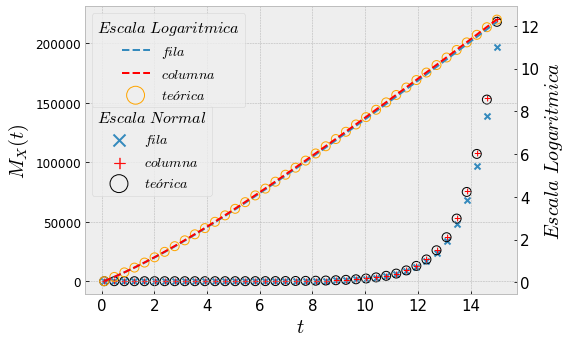
\includegraphics[width=0.49\textwidth]{Tesis UNAM/graficas/R30/Uniformidad/FGM_r30.png}}
\hfill
\subfigure{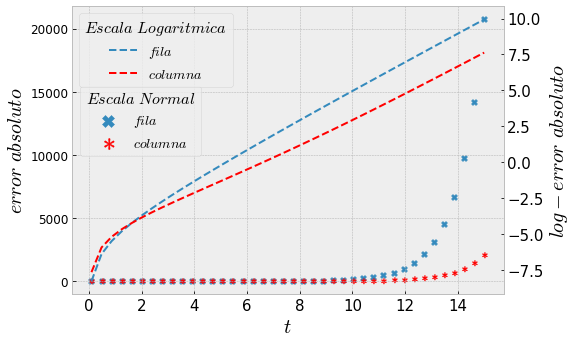
\includegraphics[width=0.49\textwidth]{Tesis UNAM/graficas/R30/Uniformidad/ErrorFGM_r30.png}}
\hfill
\caption{Comparación de la función generadora de momentos.}
\label{fig:FGM_R30}
\end{figure}


\subsubsection{Función Característica}
En la Figura \ref{fig:FC_R30} podemos ver de lado izquierdo los valores de la función característica teórica y empírica con valores $t \in [0,20] $ y de lado derecho el error absoluto entre los valores teóricos de la función y los datos simulados, de nuevo, en dos escalas. De esta manera se aprecia que, en efecto, las columnas tienen un error más pequeño para valores grandes de $t$, en este caso mayores a siete.

\begin{figure}[h!]
\hfill
\subfigure
{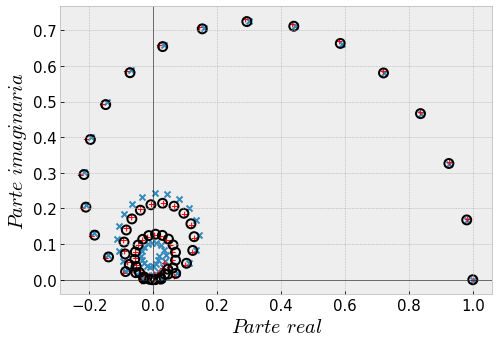
\includegraphics[width=0.39\textwidth]{Tesis UNAM/graficas/R30/Uniformidad/R30_FC.png}}
\hfill
\subfigure{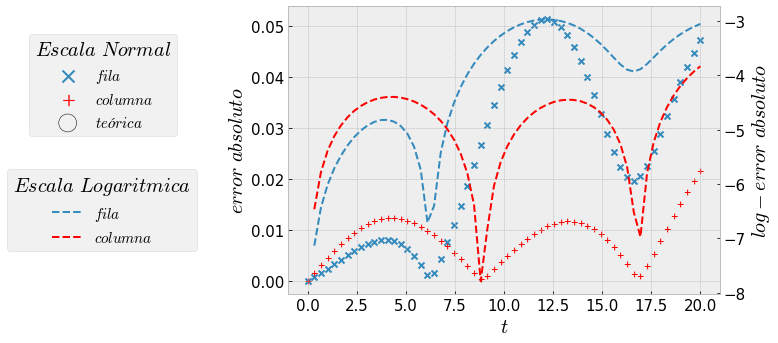
\includegraphics[width=0.59\textwidth]{Tesis UNAM/graficas/R30/Uniformidad/R30_FCError.png}}
\hfill
\caption{Comparación de la función característica.}
\label{fig:FC_R30}
\end{figure}

\subsection{Independencia}

Antes de presentar los experimentos, conviene señalar la siguiente observación:
 \begin{remark}
\label{obs:ord}
    Un reordenamiento pseudoaleatorio de los datos se puede ver como una estrategia contra la correlación de los mismos. Trabajos como \cite{Phatak1993} usan esta estrategia para dotar de independencia a datos provenientes de un mapeo logístico.
\end{remark}
Con esta idea en mente, en este experimento aplicamos dos pruebas de independencia a los datos obtenidos de la regla 30 y a un reordenamiento \footnote{El reordenamiento puede ser arbitrario pero el utilizado en este trabajo consiste en aplicar a los datos de la regla 30 el orden inducido por un conjunto de datos generados con el mapeo logístico.} de los mismos.

\subsubsection{Prueba del Coleccionista de Cupones}
Aplicando la prueba de independencia presentada en el capítulo anterior obtenemos los resultados mostrados en las Figuras \ref{fig:PCC_R30_col} y \ref{fig:PCC_R30_fila} para los desempeños de las columnas y las filas, respectivamente. De lado izquierdo, están comparadas las funciones de distribución teóricas y prácticas, mientras que de lado derecho, podemos observar la comparación entre las respectivas funciones de densidad.

\begin{figure}[h!]
\hfill
\subfigure{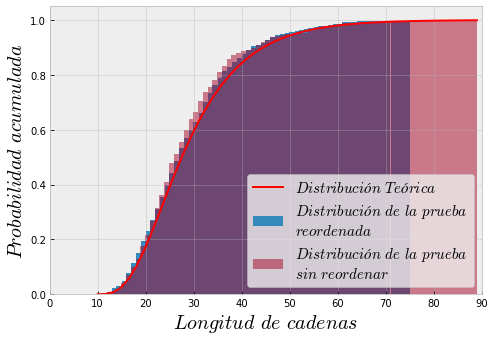
\includegraphics[width=0.49\textwidth]{Tesis UNAM/graficas/R30/Independencia/R30_col_distCCT.png}}
\hfill
\subfigure{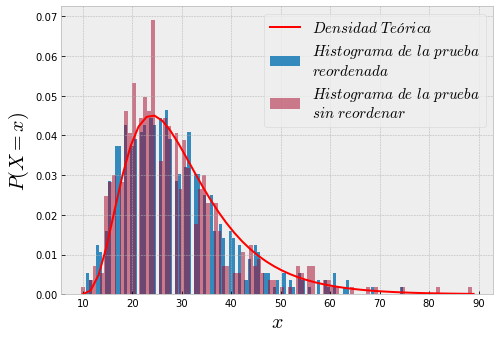
\includegraphics[width=0.49\textwidth]{Tesis UNAM/graficas/R30/Independencia/R30_col_densCCT.png}}
\hfill
\caption{Gráficas de la prueba aplicada a las columnas.}
\label{fig:PCC_R30_col}
\end{figure}

En este experimento podemos notar que el reordenamiento parece tener una ligera mejora en el desempeño de la prueba para ambos conjuntos de datos.
\begin{figure}[h!]
\hfill
\subfigure{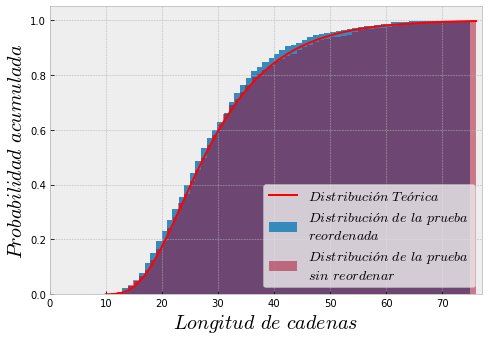
\includegraphics[width=0.49\textwidth]{Tesis UNAM/graficas/R30/Independencia/R30_fila_distCCT.png}}
\hfill
\subfigure{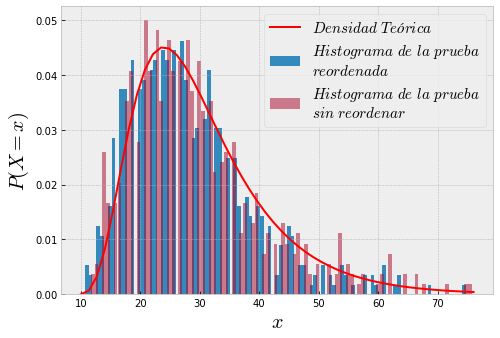
\includegraphics[width=0.49\textwidth]{Tesis UNAM/graficas/R30/Independencia/R30_fila_densCCT.png}}
\hfill
\caption{Gráficas de la prueba aplicada a las filas.}
\label{fig:PCC_R30_fila}
\end{figure}

\subsubsection{Prueba Geométrica}
Ahora implementaremos la segunda prueba de independencia introducida en el capítulo anterior. Así, obtenemos resultados como los exhibidos en la Figura  \ref{fig:PG_R30} donde podemos observar la relevancia del orden de la muestra al momento de medir la independencia con esta prueba. 
\begin{figure}[h!]
\hfill
\subfigure[Columnas]{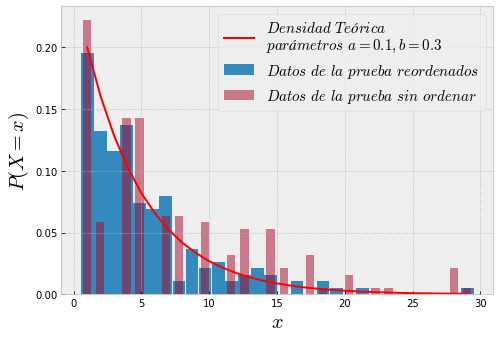
\includegraphics[width=0.49\textwidth]{Tesis UNAM/graficas/R30/Independencia/R30_col_PG.png}}
\hfill
\subfigure[Filas]{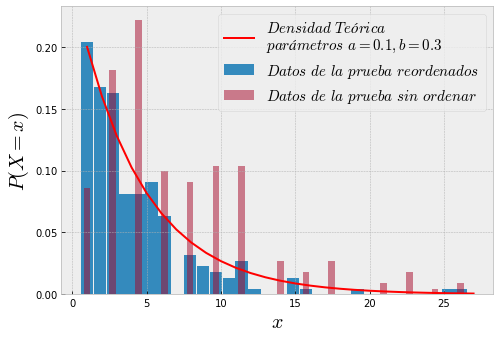
\includegraphics[width=0.49\textwidth]{Tesis UNAM/graficas/R30/Independencia/R30_fila_PG.png}}
\hfill
\caption{Gráficas de la prueba aplicada a las columnas y filas.}
\label{fig:PG_R30}
\end{figure}

\section{Mapeo tienda}
\subsection{Convergencia}
Es posible verificar numéricamente que la distribución uniforme es atractora bajo el mapeo tienda, esto es que dada cualquier distribución inicial $Y_0$ con soporte en $[0,1]$, si definimos $$Y_n = \phi(Y_{n-1})$$ con $\phi$ la función de evolución del mapeo tienda (\ref{eq:tent}), entonces la sucesión $\{Y_n\}$ converge a $X\sim U[0,1]$ en distribución. Usando la igualdad \ref{eq:dens_Y_tent}, dada una densidad inicial $f_{Y_{0}}$, podemos construir $f_{Y{_n}}$ de la siguiente manera.
\begin{equation}
    f_{Y_{n}}(y)=\frac{1}{2}\left[f_{Y_{n-1}}\left(\frac{y}{2}\right)+f_{Y_{n-1}}\left(1-\frac{y}{2}\right)\right]
    \label{eq:dens_Yn_tent}
\end{equation}
Para este experimento usaremos una distribución inicial $Beta(2,2)$ que, en efecto, tiene soporte en $[0,1]$.

% \begin{figure}[h]
%     \centering
%     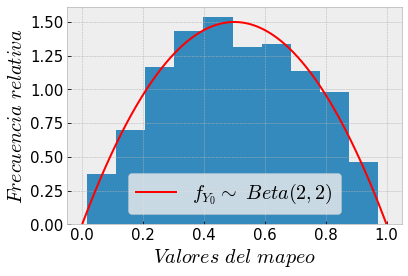
\includegraphics[width=0.49\textwidth]{Tesis UNAM/graficas/Tent/Convergencia/TentConv_histogramaIt0.png}
%     \caption{Distribución incial}
%     \label{fig:tent_it0}
% \end{figure} 

En la Figura \ref{fig:tent_conv} podemos apreciar las funciones de densidad teóricas graficadas junto a la simulación numérica de los datos en cada iteración de la sucesión $\{Y_n\}$ hasta $n=4$ en donde podemos apreciar la convergencia de las funciones de densidad teóricas $f_Y{_n}$ obtenidas con la igualdad \ref{eq:dens_Yn_tent} para cada iteración del mapeo.

% \begin{figure}[ht!]
%      \begin{center}
% %
%         \subfigure[Iteración 1]{%
%             \label{fig:first}
%             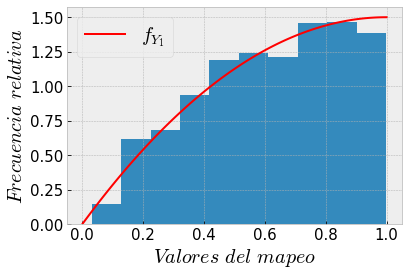
\includegraphics[width=0.49\textwidth]{Tesis UNAM/graficas/Tent/Convergencia/TentConv_histogramaIt1.png}
%         }%
%         \subfigure[Iteración 2]{%
%            \label{fig:second}
%            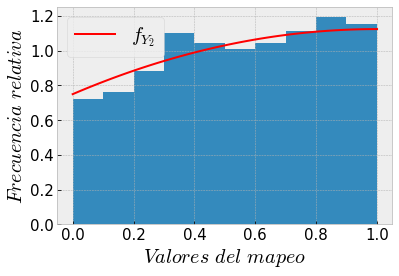
\includegraphics[width=0.49\textwidth]{Tesis UNAM/graficas/Tent/Convergencia/TentConv_histogramaIt2.png}
%         }\\ %  ------- End of the first row ----------------------%
%         \subfigure[Iteración 3]{%
%             \label{fig:third}
%             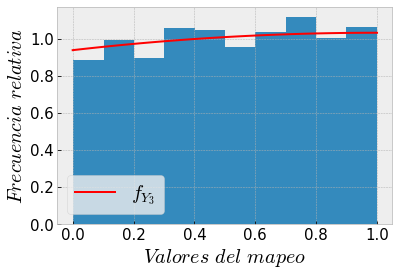
\includegraphics[width=0.49\textwidth]{Tesis UNAM/graficas/Tent/Convergencia/TentConv_histogramaIt3.png}
%         }%
%         \subfigure[Iteración 4]{%
%             \label{fig:fourth}
%             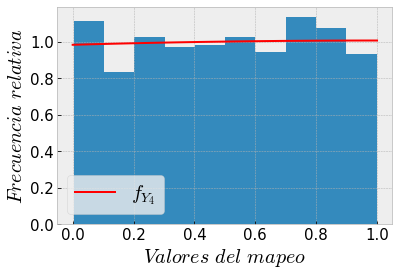
\includegraphics[width=0.49\textwidth]{Tesis UNAM/graficas/Tent/Convergencia/TentConv_histogramaIt4.png}
%         }%
% %
%     \end{center}
%     \caption{%
%         Convergencia del mapeo tienda
%      }%
%    \label{fig:Tent_conv}
% \end{figure}

\begin{figure}[h]
    \centering
    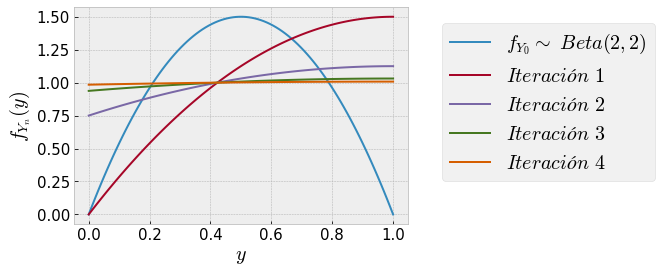
\includegraphics[width=0.80\textwidth]{Tesis UNAM/graficas/Tent/Convergencia/TentConv_Iteraciones.png}
    \caption{Convergencia del mapeo tienda a la densidad uniforme.}
    \label{fig:tent_conv}
\end{figure} 


\subsection{Uniformidad}
En esta sección analizaremos los histogramas de los datos así como sus funciones representativas con el objetivo de medir la uniformidad de los datos obtenidos.
\subsubsection{Histograma}
Una vez implementado el mapeo \ref{eq:tent} podemos obtener un conjunto de datos con el histograma presentado en la Figura \ref{fig:hist_tent}. En ella podemos empezar a apreciar que los datos sugieren tener una distribución uniforme en el intervalo $[0,1]$.

\begin{figure}[h]
    \centering
    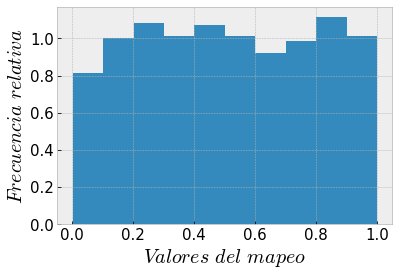
\includegraphics[width=7cm]{Tesis UNAM/graficas/Tent/Uniformidad/Tent_histograma.png}
    \caption{Histograma del mapeo}
    \label{fig:hist_tent}
\end{figure} 

\subsubsection{Momentos}
La comparación de los momentos téoricos y los numéricos obtenidos de los datos esta en la Figura \ref{fig:momentos_tent} donde podemos ver de lado derecho que el error absoluto entre los datos y el valor real es del orden de $10^{-3}$ al igual que en la Regla 30.
% Momentos
\begin{figure}[h!]
\hfill
\subfigure{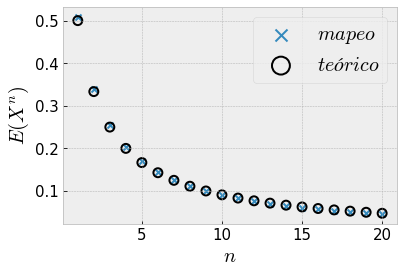
\includegraphics[width=0.48\textwidth]{Tesis UNAM/graficas/Tent/Uniformidad/Tent_Momentos.png}}
\hfill
\subfigure{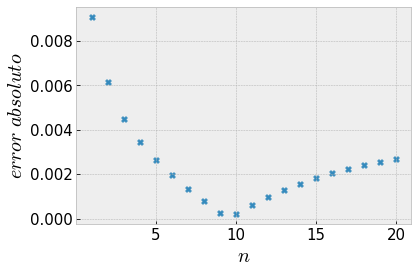
\includegraphics[width=0.49\textwidth]{Tesis UNAM/graficas/Tent/Uniformidad/Tent_MomentosError.png}}
\hfill
\caption{Comparacion de los momentos y el error absoluto.}
\label{fig:momentos_tent}
\end{figure}

\subsubsection{Función Generadora de Momentos}
Los datos correspondientes a la Función Generadora de momentos estan ilustrados en la Figura \ref{fig:FGM_tent} en la cual podemos observar que los datos se ajustan muy bien para valores de $t$ pequeños, mientras que para valores grandes de $t$ el error tiende a incrementar. Este comportamiento es de esperarse pues recordemos que la función generadora de momentos de una variable aleatoria uniforme no está acotada. 

\begin{figure}[h!]
\hfill
\subfigure{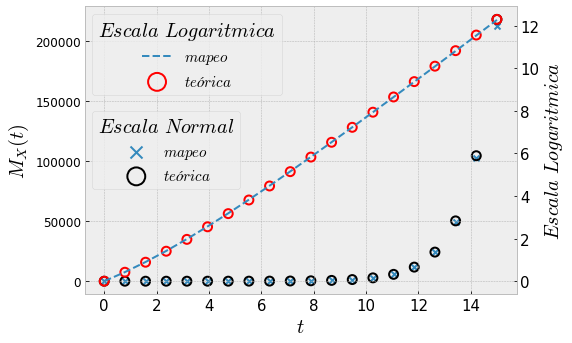
\includegraphics[width=0.49\textwidth]{Tesis UNAM/graficas/Tent/Uniformidad/Tent_FGM.png}}
\hfill
\subfigure{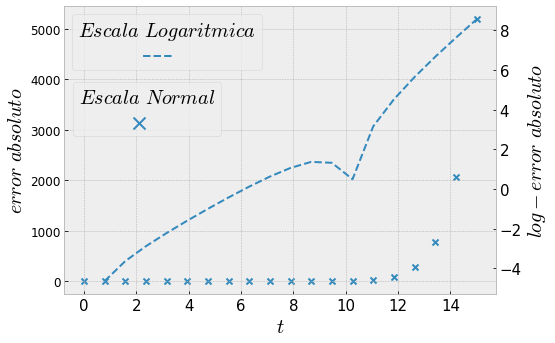
\includegraphics[width=0.49\textwidth]{Tesis UNAM/graficas/Tent/Uniformidad/Tent_ErrorFGM.png}}
\hfill
\caption{Comparación de las FGM.}
\label{fig:FGM_tent}
\end{figure}
\subsubsection{Función Característica}
En cuanto al comportamiento de la función característica, los resultados se despliegan en la Figura \ref{fig:FC_tent}, en la cual observamos que los valores esta muy cerca del valor teórico y debido a que la función tiende a acumularse en el origen, el error absoluto graficado en la derecha de la figura oscila en valores de orden $10^{-2}$.
\begin{figure}[h!]
\hfill
\subfigure{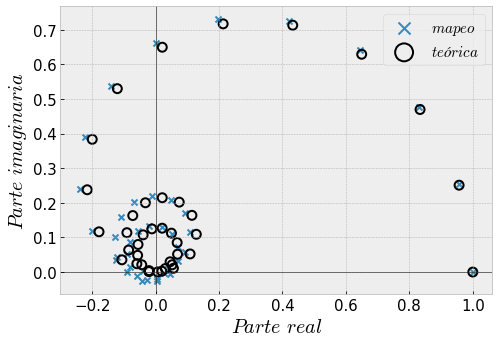
\includegraphics[width=0.49\textwidth]{Tesis UNAM/graficas/Tent/Uniformidad/Tent_FC.png}}
\hfill
\subfigure{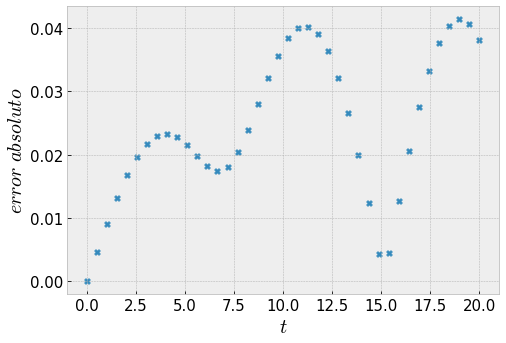
\includegraphics[width=0.49\textwidth]{Tesis UNAM/graficas/Tent/Uniformidad/Tent_FCError.png}}
\hfill
\caption{Comparación de las FC.}
\label{fig:FC_tent}
\end{figure}

\subsection{Independencia}
\subsubsection{Prueba del Coleccionista de Cupones}

Al aplicar la prueba a los datos obtenidos con el mapeo, tenemos resultados muy favorables, visibles en la Figura \ref{fig:PCC_tent}, donde podemos también apreciar una ligera mejora en el desempeño de la prueba para los valores reordenados. 
\begin{figure}[h!]
\hfill
\subfigure{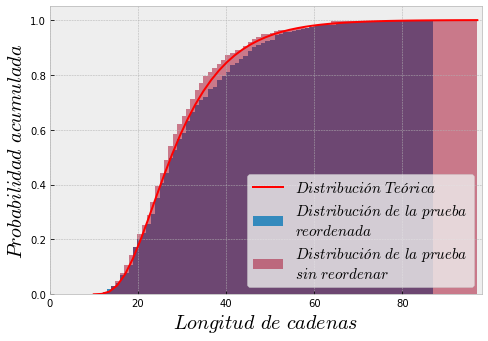
\includegraphics[width=0.49\textwidth]{Tesis UNAM/graficas/Tent/Independencia/Tent_dsit_CCT.png}}
\hfill
\subfigure{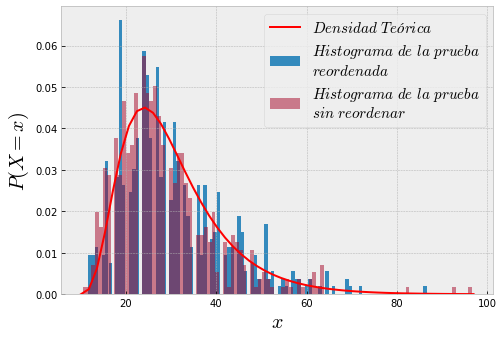
\includegraphics[width=0.49\textwidth]{Tesis UNAM/graficas/Tent/Independencia/Tent_dens_CCT.png}}
\hfill
\caption{Gráficas de la prueba aplicada al mapeo.}
\label{fig:PCC_tent}
   \end{figure}
\subsubsection{Prueba Geométrica}
En cuanto a la segunda prueba de independencia, podemos apreciar que los datos reordenados, sin duda, tienen una prueba más satisfactoria. 
\begin{figure}[h!]
    \centering
    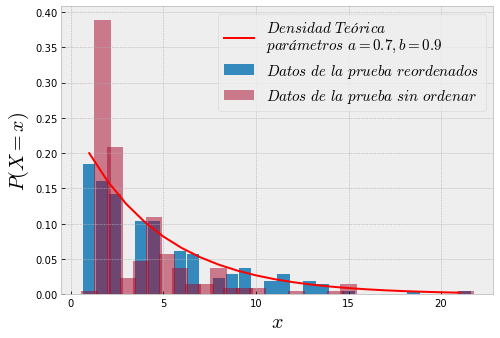
\includegraphics[width=7cm]{Tesis UNAM/graficas/Tent/Independencia/Tent_PG.png}
    \caption{Gráficas de la prueba aplicada al mapeo}
    \label{fig:PG_tent}
\end{figure} 


\section{Mapeo Logístico}

En otros trabajos se ha usado el mapeo Logístico para generar números uniformes en $[0,1]$ aún cuando la secuencia no es uniforme y necesita una transformación \cite{Phatak1993}. En este trabajo usamos la \cref{prop:inv} para obtener datos uniformes en el intervalo $[0,1]$. 
\subsection{Convergencia}

Como ya vimos en la \cref{prop:log_unif}, la distribución $Beta(\frac{1}{2},\frac{1}{2})$ es invariante al mapeo logístico. Pero la incógnita de que sea una distribución atractora sigue en pie. En esta sección veremos numéricamente que la respuesta a esa incógnita parece ser afirmativa. 

Usando la igualdad obtenida en la \cref{prop:log_unif}
\begin{align*}
f_Y(y) =\frac{1}{4} (1 - y)^{-1/2} \left[ f_X\left( \frac{1 - \sqrt{1 - y}}{2} \right) + f_X\left( \frac{1 + \sqrt{1 - y}}{2} \right) \right] 
\end{align*}
dada una densidad inicial $f_{Y_{0}}$,  si definimos $$Y_n = \phi(Y_{n-1})$$ con $\phi$ la función de evolución del mapeo logístico (\ref{eq:log}), podemos construir $f_{Y{_n}}$ de la siguiente manera:

\begin{align*}
f_{Y_n}(y) =\frac{1}{4} (1 - y)^{-1/2} \left[ f_{Y_{n-1}}\left( \frac{1 - \sqrt{1 - y}}{2} \right) + f_{Y_{n-1}}\left( \frac{1 + \sqrt{1 - y}}{2} \right) \right].
\end{align*}
En este experimento se usó una distribución inicial triangular con parámetros $(0,\frac{1}{2},1)$.

En la \cref{fig:log_conv} se puede ver que a medida que avanzan las iteraciones del mapeo, la función de densidad es cada vez más cercana a una densidad $Beta(\frac{1}{2},\frac{1}{2})$.

\begin{figure}[h]
    \centering
    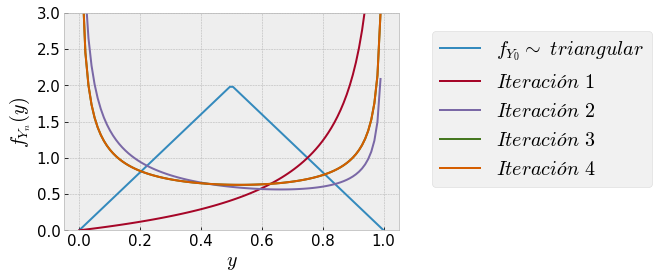
\includegraphics[width=0.80\textwidth]{Tesis UNAM/graficas/Logist/Convergencia/LogConv_Iteraciones.png}
    \caption{Convergencia del mapeo logistico a la distribución $Beta(\frac{1}{2},\frac{1}{2})$.}
    \label{fig:log_conv}
\end{figure} 


\subsection{Uniformidad}
\subsubsection{Histograma}
Una vez que obtenemos los datos del mapeo logístico y usamos la \cref{prop:inv} para obtener datos uniformes, su histograma se ve como la \cref{fig:hist_Log}, en la cual se puede apreciar como en efecto, los datos se distribuyen uniformemente en el intervalo $[0,1]$.
\begin{figure}[h!]
    \centering
    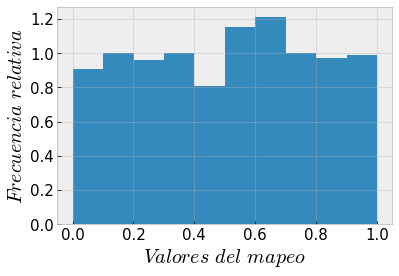
\includegraphics[width=7cm]{Tesis UNAM/graficas/Logist/Uniformidad/LogUnif_histograma.png}
    \caption{Histograma del mapeo ``uniformizado''.}
    \label{fig:hist_Log}
\end{figure} 

\subsubsection{Momentos}
    La \Cref{fig:Log_momentos} compara los momentos teóricos con los númericos. De lado derecho podemos ver el error absoluto de los momentós numéricos, en donde podemos ver como para valores pequeños de $n$ el error es igualmente pequeño alcanzando un máximo al rededor del nueve para lego tener una tendencia decreciente en la medida en que aumenta $n$.
\begin{figure}[h!]
\hfill
\subfigure{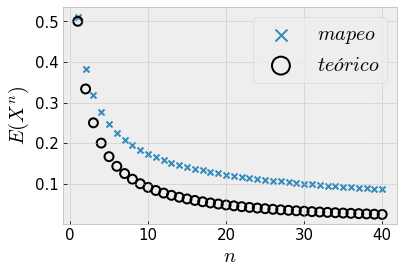
\includegraphics[width=0.49\textwidth]{Tesis UNAM/graficas/Logist/Uniformidad/Log_Momentos.png}}
\hfill
\subfigure{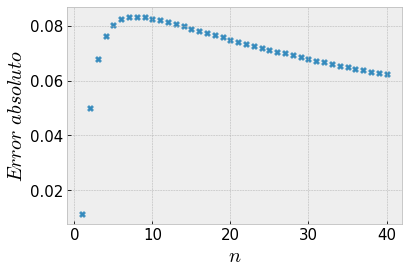
\includegraphics[width=0.49\textwidth]{Tesis UNAM/graficas/Logist/Uniformidad/Log_MomentosError.png}}
\hfill
\caption{Comparación de los momentos y el error absoluto.}
\label{fig:Log_momentos}
\end{figure}

\subsubsection{Función Generadora de Momentos}

En cuanto a la Función Generadora de Momentos, en la \Cref{fig:FGM_Log} podemos apreciar un comportamiento similar teniendo un error cercano a cero para valores de $t$ pequeños.


\begin{figure}[h!]
\hfill
\subfigure{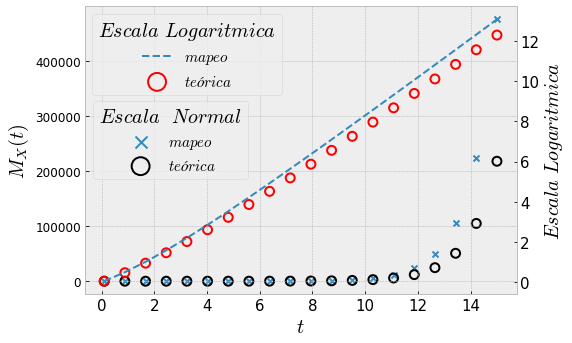
\includegraphics[width=0.49\textwidth]{Tesis UNAM/graficas/Logist/Uniformidad/Log_FGM.png}}
\hfill
\subfigure{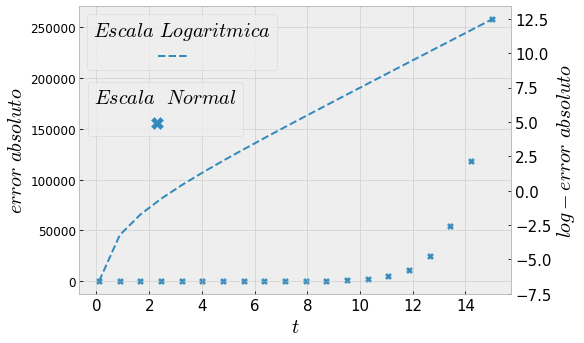
\includegraphics[width=0.49\textwidth]{Tesis UNAM/graficas/Logist/Uniformidad/Log_ErrorFGM.png}}
\hfill
\caption{Comparación de la Función Generadora de Momentos y el error absoluto con los datos obtenidos del mapeo.}
\label{fig:FGM_Log}
\end{figure}
\subsubsection{Función Característica}

La gráficas correspondientes a la función característica están en la \Cref{fig:FC_log} donde podemos ver en la gráfica izquierda los valores numéricos están distanciados de los teóricos. Sin embargo, en la gráfica del error podemos apreciar un comportamiento similar al mapeo tienda donde hay fluctuaciones del error pero también en contraste podemos ver un atenuamiento de las oscilaciones cuando $t$ crece debido a que la función característica teórica de una densidad uniforme se aglutina en el origen complejo.

\begin{figure}[h!]
\hfill
\subfigure{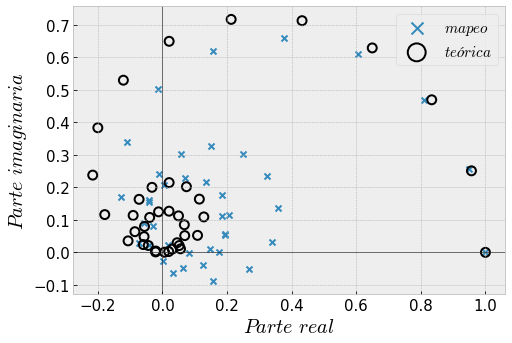
\includegraphics[width=0.49\textwidth]{Tesis UNAM/graficas/Logist/Uniformidad/Log_FC.png}}
\hfill
\subfigure{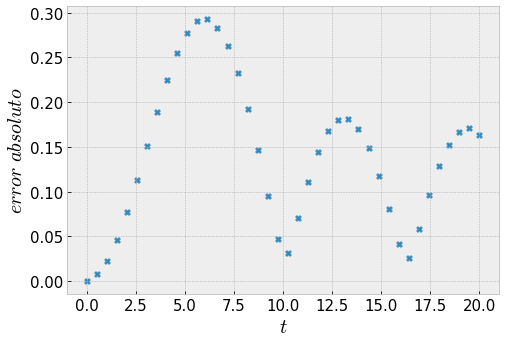
\includegraphics[width=0.49\textwidth]{Tesis UNAM/graficas/Logist/Uniformidad/Log_FCError.png}}
\hfill
\caption{Comparación de la Función Caracteristica y el error absoluto con los datos obtenidos del mapeo.}
\label{fig:FC_log}
\end{figure}

\subsection{Independencia}
\subsubsection{Prueba del Coleccionista de Cupones}

Aplicando la prueba a los datos obtenidos por el mapeo logístico tenemos los gráficos presentados en la \Cref{fig:PCC_log}, en la cual podemos ver en la gráfica izquierda correspondiente a la probabilidad acumulada cómo los datos reordenados tienen una mejora para valores grandes.
\begin{figure}[h!]
\hfill
\subfigure{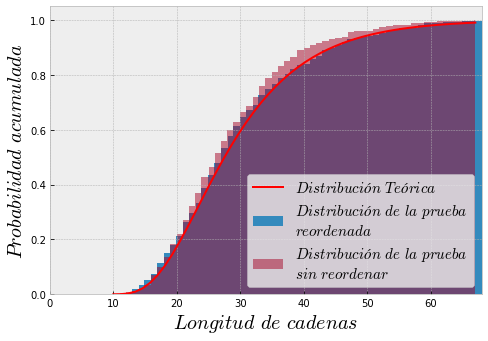
\includegraphics[width=0.49\textwidth]{Tesis UNAM/graficas/Logist/Independencia/log_dist_CCT.png}}
\hfill
\subfigure{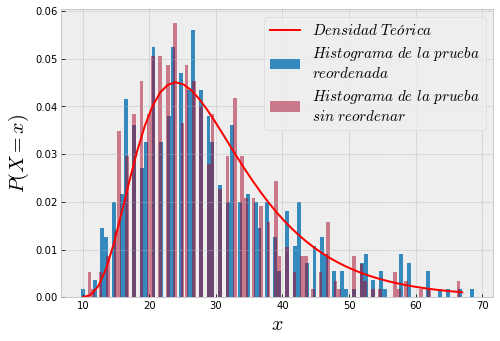
\includegraphics[width=0.49\textwidth]{Tesis UNAM/graficas/Logist/Independencia/Log_dens_CCT.png}}
\hfill
\caption{Gráficas de la prueba aplicada al mapeo.}
\label{fig:PCC_log}
\end{figure}
\subsubsection{Prueba Geométrica}
Los resultados de la prueba geométrica están desplegados en la gráfica de la \Cref{fig:PG_log}, en la cual podemos ver claramente como el reordenamiento de los datos es un método sencillo y efectivo para la obtención de datos independientes. 
\begin{figure}[h!]
    \centering
    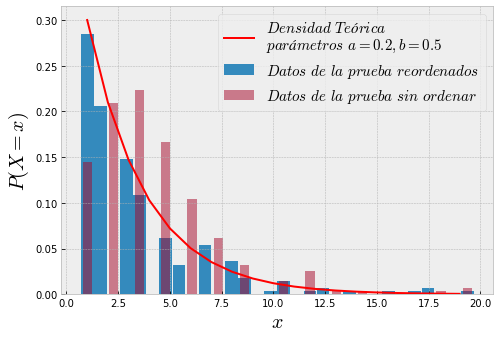
\includegraphics[width=7cm]{Tesis UNAM/graficas/Logist/Independencia/Log_PG.png}
    \caption{Gráficas de la prueba aplicada al mapeo}
    \label{fig:PG_log}
\end{figure} 

\end{document}
